\documentclass[conference, twocolumn]{IEEEtran}

% ============================================================
% PACKAGES
% ============================================================
\usepackage{cite}
\usepackage{amsmath,amssymb,amsfonts}
\usepackage{graphicx}
\usepackage{textcomp}
\usepackage{xcolor}
\usepackage{hyperref}
% --- Figures / diagrams ---
\usepackage{tikz}
\usetikzlibrary{positioning, arrows.meta, shapes.geometric}
\usepackage{pgfplots}
\pgfplotsset{compat=1.18}

\begin{document}

% ============================================================
% TITLE / AUTHORS (edit as needed)
% ============================================================
\title{Object Detection: Advancing the Trade-off Between
Speed and Accuracy}

\author{
\IEEEauthorblockN{Kumar Prateek}
\IEEEauthorblockA{
\textit{Department of Information Technology}\\
\textit{Indian Institute of Information Technology, Allahabad}\\
Prayagraj, India\\
iit2023087@iiita.ac.in}
}

\maketitle

% ============================================================
% ABSTRACT
% ============================================================
\begin{abstract}
Object detection seeks to determine \emph{what} objects appear in
an image and \emph{where} they are located, making it a central
capability for perception systems in robotics, automation, and
visual analytics. This paper reviews how object detection has
progressed from classical computer-vision pipelines---built around
hand-crafted features, sliding windows, and heuristic proposal
mechanisms---to modern deep learning approaches that learn both
features and decision rules end-to-end. Rather than presenting this
history as a single upward trend in benchmark scores, we structure
the discussion around an enduring constraint: improving precision
often increases computational cost, while improving runtime speed
often reduces representational power. We analyze how different
generations of detectors navigated this tension, why it repeatedly
re-emerges under real deployment constraints, and how recent
architectures attempt to narrow the gap through better multi-scale
representations and more efficient computation. The result is a
framework for interpreting detector design choices as trade-offs
between accuracy-centric and latency-centric objectives, and a
motivation for hybrid strategies that aim to improve both metrics
without simply scaling model size.
\end{abstract}

% ============================================================
% INDEX TERMS
% ============================================================
\begin{IEEEkeywords}
Object Detection, Speed--Accuracy Trade-off, mean Average Precision,
Frames Per Second, Localization, Classification
\end{IEEEkeywords}

% ============================================================
% I. INTRODUCTION
% ============================================================
\section{Introduction}

Object detection is commonly defined as the joint task of
\textit{classification} and \textit{localization}. Given an image,
a detector must identify instances of predefined categories and
estimate their spatial extent, most often as axis-aligned bounding
boxes. Unlike image-level classification---which returns a fixed-size
label vector---detection produces a variable-length set of outputs:
the number of objects is unknown beforehand, objects may overlap,
and instances can appear at drastically different scales within the
same scene. As a consequence, detection models must learn both
discriminative semantics (to decide \emph{what} an object is) and
fine-grained spatial reasoning (to decide \emph{where} it is).

The practical importance of this capability is easy to justify.
Autonomous vehicles and mobile robots require low-latency perception
to support closed-loop control. Surveillance and industrial
inspection require high precision to avoid costly false alarms and
misses, while still processing continuous streams. These demands
are not independent: the fastest detector is unusable if it misses
critical objects, and the most accurate detector is impractical if
it cannot keep up with real-time inputs. This coupling leads to the
core tension that frames this paper: optimizing detection accuracy
and inference speed together is historically difficult.

\subsection{The Balancing Act: mAP versus FPS}

The most widely reported accuracy metric is mean Average Precision
(mAP). At a high level, mAP aggregates performance over a
precision--recall curve and averages across classes (and, in modern
benchmarks, across multiple IoU thresholds). It therefore rewards
correct classification, tight box alignment with ground truth, and
robustness across occlusion levels and object sizes. Improvements
in mAP typically reflect fewer false positives, fewer missed
detections, and more accurate localization.

Speed is commonly reported as Frames Per Second (FPS), i.e., how
many images can be processed per second during inference on a given
hardware configuration. FPS is closely related to latency: higher
FPS generally implies that the detector can support higher-rate
inputs without buffering delays.

Achieving high mAP and high FPS simultaneously is challenging
because the mechanisms that raise accuracy frequently increase
compute. Deeper backbones expand feature capacity but add FLOPs.
Multi-scale fusion improves small-object performance but introduces
additional pathways and operations. Iterative refinement strategies
can tighten localization but impose sequential steps that do not
parallelize cleanly. Conversely, aggressive efficiency strategies
can remove the spatial detail or semantic richness that detection
requires. Downsampling early reduces cost but harms small-object
localization; narrow feature channels and simplified heads can speed
up inference but reduce discrimination in crowded scenes.

The remainder of this article traces the evolution of object
detection using this lens: each era is discussed in terms of how it
positions itself on the speed--precision curve, what compromises it
accepts, and which architectural ideas attempt to move the frontier
rather than simply choosing one end of the trade-off.


% ============================================================
% PAGE 2 — THE PRE-DEEP LEARNING ERA (TRADITIONAL METHODS)
% Paste this BELOW Page 1 content and BEFORE \begin{thebibliography}
% ============================================================

\section{The Pre-Deep Learning Era (Traditional Methods)}

Before deep learning reshaped visual recognition around 2012,
object detection pipelines were largely engineered by hand.
A typical system combined (i) a manually designed feature
representation, (ii) a classifier such as a linear SVM, and
(iii) a search strategy, often sliding windows across an image
pyramid, to locate candidate objects. This era produced several
high-impact ideas that made detection practical in real time on
CPU hardware, but it also revealed a central constraint: when
features are hand-crafted, the detector can only be as robust
as the designer's assumptions about what visual evidence
matters.


\subsection{Viola--Jones: Real-Time Face Detection with Haar Features}

A major milestone was the Viola--Jones framework for
near real-time face detection \cite{viola2001rapid}. Its core
feature family consisted of \textit{Haar-like} intensity
differences computed over adjacent rectangular regions (e.g.,
two-rectangle and three-rectangle patterns). Two algorithmic
choices made these features computationally attractive on CPUs.

First, the \textit{integral image} representation allowed
rectangle sums to be computed in constant time independent of
rectangle size. As a result, a large number of Haar-like
features could be evaluated quickly for each candidate window.
Second, Viola--Jones used AdaBoost to select a small subset of
high-utility features from a much larger pool, simultaneously
forming a strong classifier from many weak learners. The final
system used a \textit{cascade of classifiers}
\cite{viola2004robust}: early stages were deliberately cheap
and rejected most background windows, while later stages were
more expressive and processed only the surviving candidates.
This cascade structure directly targeted runtime constraints
and remains conceptually influential in modern ``early-exit''
and pruning strategies.

\subsection{HOG + SVM: Gradient Structure for Pedestrian Detection}

While Haar features were effective for faces under relatively
controlled appearance variation, more general object categories
often required descriptors that were less sensitive to raw
illumination and more aligned with shape. Histogram of Oriented
Gradients (HOG) \cite{dalal2005histograms} addressed this by
encoding local edge structure: an image window was divided into
cells, each cell accumulated a histogram of gradient
orientations, and neighboring cells were grouped into blocks
for contrast normalization. The resulting descriptor captured
coarse contour geometry while reducing sensitivity to lighting
changes.

HOG was frequently paired with a linear SVM trained on positive
windows (containing pedestrians) and negative windows
(background). Detection proceeded by evaluating the SVM score
over sliding windows at multiple scales. Although sliding
window search is computationally expensive, the combination of
a linear classifier and structured gradient features produced
strong pedestrian results for its time and became a standard
baseline for years. Importantly, HOG illustrated a recurring
theme in pre-deep-learning detection: strong performance often
came from designing features that aligned well with the
dominant visual statistics of a specific object class.

\subsection{DPM: Deformable Part-Based Models}

Deformable Part-based Models (DPMs) represented the high-water
mark of traditional detection before deep networks became
dominant \cite{felzenszwalb2010object}. DPMs treated an object
as a collection of parts arranged in a deformable configuration.
A typical formulation included (i) a \textit{root} filter that
roughly captured the object, (ii) several higher-resolution
\textit{part} filters that captured local structure, and
(iii) deformation costs that penalized deviations of parts from
their ideal relative positions.

The strength of DPMs was their explicit modeling of intra-class
variation: a pedestrian can be detected even when limbs shift
due to pose changes, and an object can be recognized despite
partial occlusion if enough parts match. Training was commonly
done with latent SVM techniques, where part placements acted as
latent variables. With carefully tuned HOG features, DPMs
achieved state-of-the-art results on benchmarks like PASCAL VOC
for several years, and they introduced ideas---compositional
structure, mixtures, and deformation tolerance---that continue
to influence later architectures.

\subsection{Limitations of Hand-Crafted Pipelines}

Despite their elegance and engineering efficiency, traditional
detectors eventually reached a hard ceiling in precision on
complex real-world imagery. The bottleneck was not only
computation; it was \textit{representation}. Hand-crafted
features such as Haar and HOG encode specific low-level cues
(edges, gradients, intensity contrasts) that may be diagnostic
in controlled settings, yet they struggle to express high-level
semantics, texture diversity, and context. As datasets became
larger and scenes more varied---with cluttered backgrounds,
unusual viewpoints, heavy occlusion, and long-tailed
appearance variation---the gap between what the features could
describe and what the task demanded widened. This mismatch set
the stage for end-to-end learned representations, where feature
extractors are optimized jointly with the detector rather than
fixed in advance.



% ============================================================
% PAGE 3 — THE DEEP LEARNING REVOLUTION & TWO-STAGE DETECTORS (PART 1)
% Paste this BELOW Page 2 content and BEFORE \begin{thebibliography}
% ============================================================

\section{The Deep Learning Era: From Designed Features to Learned Features}

Around 2012, object detection research began to pivot away from
feature engineering and toward representation learning. The
catalyst was the success of AlexNet \cite{krizhevsky2012imagenet}
in large-scale recognition, which demonstrated that deep
convolutional neural networks (CNNs) could learn hierarchical
visual features directly from data. For detection, this was a
fundamental change in \emph{where} progress came from: rather
than inventing better gradient or texture descriptors by hand,
researchers could train a feature extractor whose internal
filters adapt to the statistics of real images.

This shift mattered because the classical ceiling was largely a
representation ceiling. Hand-crafted descriptors typically
capture a narrow family of cues (edges, corners, oriented
gradients) and rely on heuristics to gain invariance to
viewpoint, occlusion, clutter, and illumination changes. CNN
features, in contrast, can jointly learn low-level structure
and high-level semantics, allowing the same backbone to support
both category discrimination and localization-sensitive cues.
However, early deep detectors still faced an expensive search
problem: \emph{which} image regions should be evaluated by the
CNN? The two-stage detector emerged as the dominant answer,
prioritizing precision through candidate selection followed by
fine-grained classification.

\subsection{Two-Stage Detectors (The Precision Pioneers)}

The defining idea of two-stage detection is to separate the
pipeline into: (i) proposing a limited set of candidate regions
that are likely to contain objects, and (ii) classifying and
refining those candidates with a stronger model. This
decomposition reduces the need to score an enormous number of
sliding windows, and it allocates high-capacity computation to
a smaller set of plausible object locations. In practice,
two-stage designs became known for strong mAP, especially when
precise localization is required, albeit often at a higher
latency than single-stage alternatives.

\subsubsection{R-CNN: Regions with CNN Features}

R-CNN \cite{girshick2014rich} was the first widely influential
detector to show that CNN features could dramatically improve
detection quality. Its workflow can be summarized as follows.

\textit{(1) Region generation.} R-CNN uses Selective Search
\cite{uijlings2013selective} to compute roughly 2\,000
category-agnostic proposals per image. Selective Search groups
superpixels by similarity, producing a diverse set of
rectangular regions spanning multiple scales and aspect ratios.
This step is external to the CNN and typically CPU-bound.

\textit{(2) Feature extraction.} Each proposal is cropped,
resized (warped) to a fixed resolution, and forwarded through a
CNN to obtain a feature vector. This was the critical leap: the
descriptor is learned rather than designed.

\textit{(3) Classification and localization.} Linear SVMs are
trained per category to classify proposal features, and a
separate bounding box regressor adjusts each proposal toward a
tighter fit.

While this pipeline substantially improved accuracy over
traditional detectors, it was inefficient. The CNN is executed
thousands of times per image (once per proposal), and proposal
generation is itself non-trivial. As a result, R-CNN was a
precision breakthrough but not a real-time solution.

\subsubsection{Fast R-CNN: Sharing Computation with RoI Pooling}

Fast R-CNN \cite{girshick2015fast} targets R-CNN's main cost:
repeated CNN evaluation. Instead of running a CNN independently
for each proposal, Fast R-CNN runs the CNN \emph{once} on the
full image to produce a shared convolutional feature map. Each
proposal is then mapped onto this feature map, and a
\textit{Region of Interest (RoI) pooling} operation extracts a
fixed-size representation per proposal by pooling over the
corresponding spatial region.

This redesign yields two practical gains:

\textit{(i) Convolutional reuse.} Since the convolutional trunk
dominates compute, sharing it across all proposals drastically
reduces inference time relative to per-proposal CNN execution.

\textit{(ii) Joint optimization.} Fast R-CNN trains
classification and bounding-box regression end-to-end using a
single multi-task loss, aligning the learned features with
detection objectives rather than treating classification and
regression as add-on modules.

Fast R-CNN therefore preserved the two-stage philosophy while
making it substantially more efficient. Yet, it still relied on
Selective Search to generate proposals, leaving a non-learned,
CPU-heavy component in the pipeline. The next step in the
two-stage lineage was to make region proposals neural and
end-to-end trainable, further tightening the speed--precision
balance.

% ============================================================
% PAGE 4 — TWO-STAGE DETECTORS (PART 2) & THE BOTTLENECK
% Paste this BELOW Page 3 content and BEFORE \begin{thebibliography}
% ============================================================

\section{Two-Stage Detectors (Part 2) and the Bottleneck}

Fast R-CNN substantially reduced the redundant computation of
R-CNN by sharing convolutional features, but it still depended
on an external proposal generator (Selective Search). That
dependency mattered for both speed and engineering: proposal
generation was typically CPU-bound, not end-to-end trainable,
and difficult to optimize jointly with the recognition model.
Faster R-CNN \cite{ren2015faster} addressed this limitation by
bringing proposal generation inside the network.

\subsection{Faster R-CNN and the Region Proposal Network (RPN)}

Faster R-CNN replaces Selective Search with a learnable
\textit{Region Proposal Network} (RPN). After the backbone CNN
produces a convolutional feature map for the input image, the
RPN slides a small network over this feature map and predicts,
at each spatial location, a set of candidate boxes (anchors)
along with an objectness score indicating whether an anchor is
likely to contain an object. High-scoring proposals are then
passed to the second stage, where RoI-based features are used
to classify the region and refine the box coordinates.

This design yields three practical advantages:

\textit{(i) End-to-end learning.} Proposal generation becomes a
trainable component optimized jointly with detection. The model
can learn to propose regions that are useful for the final
classification and regression objectives, rather than relying
on a handcrafted grouping heuristic.

\textit{(ii) Major speed gains over CPU proposals.} The RPN runs
on the same shared CNN feature map and can be executed on the
GPU. This removes a slow external stage and makes the full
pipeline substantially faster and more hardware-friendly.

\textit{(iii) Better proposal quality.} Because proposals are
learned and can leverage deep feature semantics, they tend to be
more aligned with object boundaries than generic heuristic
regions, improving downstream classification and localization.

Despite these improvements, Faster R-CNN retains the defining
two-stage structure: it still performs proposal generation
followed by per-proposal feature extraction and classification.
This sequential organization is a central reason why two-stage
detectors often excel in mAP but frequently lag in FPS compared
to single-stage designs.

\subsection{Intersection over Union (IoU): Measuring Overlap}

A key geometric quantity in detection is \textit{Intersection
over Union} (IoU), which measures how well a predicted bounding
box aligns with a ground-truth box. Given a predicted box
$B_p$ and a ground-truth box $B_{gt}$, IoU is defined as
\begin{equation}
    \text{IoU} =
    \frac{\text{Area}(B_p \cap B_{gt})}
         {\text{Area}(B_p \cup B_{gt})}
    \label{eq:iou}
\end{equation}
IoU ranges from $0$ (no overlap) to $1$ (perfect alignment).
It appears throughout the detection pipeline in two distinct
roles.

\textit{(i) Evaluation.} Benchmarks declare a detection to be a
true positive if $\text{IoU}(B_p,B_{gt})$ exceeds a chosen
threshold. Stricter thresholds penalize imprecise localization,
which is why COCO-style evaluation (averaging across multiple
IoU thresholds) is more demanding than single-threshold
protocols.

\textit{(ii) Training and label assignment.} In two-stage
detectors, IoU is used to assign positive and negative labels
to anchors and proposals. For example, an anchor may be treated
as positive if its IoU with any ground truth exceeds a high
threshold, negative if below a low threshold, and ignored
otherwise. This creates a supervised signal for the RPN and
helps focus learning on candidate regions that plausibly
correspond to real objects.

IoU thus connects the geometry of localization to both the
training signal and the final reported performance.

\subsection{The Two-Stage Ceiling: Why FPS Remains Hard}

Even with an efficient RPN, two-stage detectors face a
structural speed ceiling for real-time video on standard
hardware. The main issue is not any single layer, but the
\textit{composition} of sequential steps and per-proposal
processing.

First, the pipeline includes at least two dependent stages
(RPN $\rightarrow$ RoI classification/regression). This limits
parallelism: the second stage cannot proceed until proposals
are generated and filtered. Second, RoI processing introduces
work proportional to the number of proposals retained. In
practice, to preserve recall, the system often keeps hundreds
of RoIs per image; each requires pooling/align operations and
several layers of computation in the head network. Third,
proposal filtering and final prediction post-processing (e.g.,
NMS) can become non-trivial overhead, especially in crowded
scenes where many candidate boxes are produced. Finally, the
data movement associated with gathering RoI features (irregular
memory access patterns) can stress memory bandwidth and reduce
effective GPU utilization, making throughput less predictable.

For these reasons, two-stage detectors often occupy the
accuracy-oriented end of the speed--precision spectrum. Their
design excels when localization quality and robustness are
prioritized, but achieving consistently high FPS for real-time
multi-stream video typically requires architectures that avoid
heavy per-proposal computation and minimize sequential
dependencies---considerations that motivate the rise of
single-stage detectors in subsequent generations.


% ============================================================
% PAGE 5 — THE SHIFT TO ONE-STAGE DETECTORS (PART 1)
% Paste this BELOW Page 4 content and BEFORE \begin{thebibliography}
% ============================================================

\section{One-Stage Detectors (Part 1): The Speed Revolution}

Two-stage detectors achieved strong precision by explicitly
separating candidate generation from classification and box
refinement. However, their proposal-centric structure tends to
create sequential dependencies and per-proposal compute that
are difficult to scale to high-FPS video workloads. One-stage
detectors emerged as a response to this bottleneck. The
one-stage philosophy discards explicit region proposals and
instead formulates detection as \textit{dense prediction}: the
network directly emits class confidences and box parameters at
many spatial locations in a single forward pass.

From an architectural standpoint, this shift replaces ``detect
a few regions very carefully'' with ``predict everywhere and
then filter.'' The approach can be interpreted as a large
multi-output regression (or classification + regression) task
performed over an image pyramid. The payoff is speed: the model
avoids a separate proposal stage and typically uses a fully
convolutional computation pattern that maps well to GPU
parallelism. The cost is that training becomes sensitive to
class imbalance (many background locations) and that early
designs struggled with precise localization for small or
crowded objects.

\subsection{YOLOv1: Unified Grid-Based Prediction}

YOLOv1 \cite{redmon2016you} introduced a highly influential
single-pass formulation. It partitions the input image into an
$S \times S$ grid. Each grid cell is responsible for predicting
a fixed number of bounding boxes and a set of class
probabilities. In a simplified view, the model outputs, per
cell, (i) box geometry parameters (center offsets and size),
(ii) a confidence value intended to reflect object presence and
box quality, and (iii) conditional class probabilities.

This design created a conceptually clean pipeline:
\textit{one network evaluation} yields a full set of detections.
Because the network sees the whole image at once, it can also
leverage global context (e.g., scene layout) in ways that
sliding-window systems cannot. Practically, YOLOv1 delivered a
large step forward in FPS compared to proposal-based methods,
making real-time detection feasible on consumer GPUs of that
time.

At the same time, the grid responsibility assignment introduces
a limitation: a single cell can only represent a small number
of objects. When multiple objects fall into the same cell or
when objects are very small relative to the cell size,
localization becomes harder. Additionally, the coarse spatial
partition can produce jitter near cell boundaries. These issues
are not fundamental to one-stage detection, but they were
prominent in early unified formulations and motivated later
improvements in multi-scale prediction and assignment
strategies.

\subsection{SSD: Multi-Scale Feature Maps for Scale Diversity}

The Single Shot MultiBox Detector (SSD) \cite{liu2016ssd}
extended the one-stage idea while directly addressing one of
YOLOv1's key weaknesses: uneven performance across object
scales. Instead of predicting from a single grid resolution,
SSD attaches lightweight detection heads to multiple feature
maps at different depths of the backbone. Shallow feature maps
retain higher spatial resolution and are used for small object
detection; deeper maps have larger receptive fields and are
used for medium and large objects.

SSD also introduced the notion of \textit{default boxes}
(also called anchor boxes) defined at each feature-map location
across multiple aspect ratios and scales. The network predicts,
for each default box, class confidences and offsets that adjust
the box toward the target object. This design increases the
variety of shapes that can be represented without requiring a
separate proposal stage, and it allows the detector to match
objects of different sizes to the most appropriate feature-map
level.

In effect, SSD preserves the single-forward-pass goal of
one-stage detection while making the prediction space more
expressive and more scale-aware. By distributing predictions
across a feature pyramid, SSD improved robustness to object
size variation and became a template for later real-time
detectors that combined multi-scale fusion with efficient head
designs.

% ============================================================
% PAGE 6 — ONE-STAGE DETECTORS (PART 2) & OVERCOMING CLASS IMBALANCE
% Paste this BELOW Page 5 content and BEFORE \begin{thebibliography}
% ============================================================

\section{One-Stage Detectors (Part 2): Overcoming Class Imbalance}

One-stage detectors achieved impressive throughput by predicting
densely in a single forward pass, but early versions often
trailed two-stage detectors in mean Average Precision (mAP).
The gap was particularly visible for small objects and crowded
scenes, where localization requires fine spatial detail and
classification must separate subtle categories under occlusion.
Understanding why this gap existed clarifies why certain
training innovations---especially Focal Loss---became decisive.

\subsection{Why Early One-Stage Models Lagged in mAP}

A central difficulty in dense prediction is that the number of
background locations dwarfs the number of foreground locations.
In anchor-based one-stage detectors, each spatial position can
have multiple anchors; across an image pyramid this can yield
tens or hundreds of thousands of candidate boxes. Only a tiny
fraction correspond to real objects. If a standard loss (e.g.,
binary cross-entropy) is applied uniformly, the training signal
is dominated by easy negatives: background anchors that the
model quickly learns to classify correctly. Once these easy
examples saturate, they still contribute a large volume of
gradient updates, which can drown out the informative signal
from rare positives and hard negatives.

This imbalance has practical consequences:

\textit{(i) Reduced recall on small objects.} Small objects
occupy fewer pixels and match fewer anchors well; they are
therefore underrepresented in the set of positive samples,
making them easier to miss during training.

\textit{(ii) Optimization instability.} When gradients are
dominated by abundant negatives, the model may converge to a
conservative regime that suppresses detections to avoid false
positives, harming recall.

\textit{(iii) Hard-example underweighting.} Background regions
that visually resemble objects (e.g., textures, repeated
patterns) are precisely the examples that should shape the
decision boundary, yet they can be numerically overshadowed by
millions of trivial negatives.

Two-stage detectors partially avoid this extreme imbalance by
filtering candidates early: an RPN proposes a manageable number
of RoIs, and the second-stage classifier sees a more balanced
set of hard negatives and positives. A key turning point for
one-stage detectors was learning how to train dense heads
without letting easy background examples dominate learning.

\subsection{RetinaNet and Focal Loss}

RetinaNet \cite{lin2017focal} demonstrated that a carefully
designed loss could close much of the accuracy gap while
retaining one-stage speed. Its main contribution was
\textit{Focal Loss}, which reshapes the classification loss so
that well-classified examples contribute less gradient, allowing
training to focus on hard misclassified examples.

Let $p \in [0,1]$ denote the model's estimated probability for
the positive class for a given anchor, and let $y \in \{0,1\}$
be the ground-truth label. Define
\begin{equation}
    p_{t} =
    \begin{cases}
        p, & \text{if } y=1\\
        1-p, & \text{if } y=0
    \end{cases}
\end{equation}
The Focal Loss is then
\begin{equation}
    \text{FL}(p_{t}) =
    -\alpha_{t}\,(1-p_{t})^{\gamma}\,\log(p_{t})
    \label{eq:focal}
\end{equation}
where $\alpha_{t}$ balances positive/negative contributions
and $\gamma \ge 0$ is the focusing parameter.

The modulating factor $(1-p_t)^{\gamma}$ is the key mechanism.
When an example is easy (high $p_t$), the term approaches zero
and the loss contribution is suppressed. When an example is
hard (low $p_t$), the factor stays near one, preserving a
strong gradient signal. In effect, Focal Loss reduces the
optimization ``attention'' paid to the overwhelming population
of trivial negatives and reallocates learning capacity to the
rare, informative cases that shape mAP: difficult foregrounds,
confusing backgrounds, and borderline localization scenarios.
This made one-stage training far more competitive without
reintroducing proposal stages.

\subsection{Evolution of the YOLO Family (v2 to v8)}

In parallel with RetinaNet, the YOLO line evolved through a
sequence of practical refinements aimed at improving mAP while
maintaining real-time FPS. YOLOv2 \cite{redmon2017yolo9000}
introduced stronger backbones and more stable training recipes
(e.g., anchor priors and multi-scale training), improving both
recall and localization. YOLOv3 \cite{redmon2018yolov3}
strengthened multi-scale prediction by detecting at multiple
feature-map resolutions, improving performance on smaller
objects without sacrificing throughput.

Later generations emphasized backbone efficiency and training
stability. YOLOv4 \cite{bochkovskiy2020yolov4} consolidated a
large set of ``bag-of-freebies'' and ``bag-of-specials'' such
as mosaic augmentation and improved feature aggregation,
pushing mAP upward at minimal inference cost. Modern YOLO
implementations also adopted backbones built around Cross-Stage
Partial connections (CSPDarknet) \cite{wang2020cspnet}, which
improve gradient flow and reduce redundant computation, helping
maintain high FPS at higher accuracy regimes.

More recent designs (e.g., YOLOv7 \cite{wang2023yolov7} and
YOLOv8 \cite{jocher2023yolov8}) continue this trend with
careful architectural scaling, improved label assignment, and
increasing interest in anchor-free or anchor-light heads that
reduce hyperparameter sensitivity to anchor design. Across
versions, the YOLO family illustrates a broad pattern: real
progress comes not from a single change, but from coordinated
improvements in backbone capacity, multi-scale representation,
loss design, and assignment strategy that jointly push the
speed--precision curve outward.

% ============================================================
% PAGE 7 — THE MODERN ERA: TRANSFORMERS AND ATTENTION
% Paste this BELOW Page 6 content and BEFORE \begin{thebibliography}
% ============================================================

\section{The Modern Era: Transformers and Attention}

As convolutional backbones and feature-pyramid designs matured,
a recurring limitation became clear: convolution is inherently
local. Even with deep stacks and large receptive fields, CNNs
primarily aggregate information through repeated neighborhood
operations. This inductive bias is powerful for texture and
local structure, but it can make it difficult to model
long-range interactions explicitly (e.g., relating distant
parts of an object, or reasoning about context across a scene).
The modern era of detection therefore saw a decisive shift
toward \textit{attention mechanisms}, which provide a direct
way to connect distant regions and compute context-aware
representations.

\subsection{DETR: Adapting Transformers for Object Detection}

DETR (DEtection TRansformer) \cite{carion2020end} introduced a
transformer-based formulation that reframed detection as a
direct prediction problem rather than a pipeline of handcrafted
subsystems. DETR combines three building blocks:

\textit{(i) A CNN backbone} produces a spatial feature map from
the input image.

\textit{(ii) A transformer encoder--decoder} performs global
reasoning. The encoder applies self-attention over the entire
feature map (after positional encoding), enabling each location
to exchange information with all others. The decoder consumes a
fixed set of learned \textit{object queries}, where each query
is intended to represent one potential object instance.

\textit{(iii) A prediction head} maps each decoded query to a
class label (including a ``no-object'' class) and bounding box
coordinates.

Unlike anchor-based detectors that generate many candidates per
pixel location, DETR produces a \emph{fixed-size} set of
predictions. This small design choice has large consequences:
it pushes instance selection into the learning problem and
reduces reliance on post-processing heuristics.

\subsection{Bipartite Matching and Direct Set Prediction}

The mechanism that makes DETR workable is \textit{bipartite
matching} between predicted objects and ground-truth objects.
Because DETR outputs an unordered set of predictions, training
requires a way to align predictions with ground truth without
imposing a hand-designed ordering. DETR uses a one-to-one
assignment computed by solving a minimum-cost matching problem
(often described as Hungarian matching).

Let the ground-truth set be $\mathcal{G}=\{g_j\}_{j=1}^{M}$,
and the model output be $\mathcal{P}=\{p_i\}_{i=1}^{N}$ with a
fixed $N$ (typically $N \ge M$). A cost function
$\mathcal{C}(p_i, g_j)$ measures how well prediction $i$ matches
ground-truth object $j$ (combining classification mismatch and
box mismatch). The matching selects a permutation $\pi$
minimizing total cost:
\begin{equation}
    \pi^{*} = \arg\min_{\pi}
    \sum_{j=1}^{M} \mathcal{C}\bigl(p_{\pi(j)},\, g_j\bigr)
\end{equation}
Once this one-to-one mapping is established, the loss is
computed on matched pairs, and the remaining unmatched
predictions are trained toward the ``no-object'' class.

This set-prediction view eliminates two hand-designed
components that were historically central to detectors:

\textit{(i) Anchor boxes.} DETR does not require a library of
predefined box shapes. The decoder queries learn to represent
object hypotheses directly, and box coordinates are regressed
without anchor priors.

\textit{(ii) Non-Maximum Suppression (NMS).} Because the model
is trained with a one-to-one matching objective, it is
explicitly discouraged from producing duplicate detections for
the same object. In principle, this removes the need for NMS,
which in classical pipelines is used to suppress multiple
overlapping predictions that refer to a single instance.

The conceptual simplification is significant: detection becomes
``predict a set'' rather than ``predict many candidates then
prune.'' In practice, the DETR family also exposed new
challenges, such as convergence speed and the computational
cost of global attention on high-resolution feature maps, which
motivated more efficient transformer designs for vision.

\subsection{Swin Transformers: Hierarchical Efficiency for Vision}

Swin Transformers \cite{liu2021swin} introduced a hierarchical
vision transformer architecture that makes attention more
computationally practical for dense visual tasks such as
detection. The key idea is \textit{window-based} self-attention:
instead of computing attention globally across all tokens,
Swin computes self-attention within local windows, drastically
reducing complexity. To prevent windows from becoming isolated,
Swin alternates between regular windows and \textit{shifted}
windows so that information can flow across window boundaries
over successive layers.

Equally important, Swin builds a multi-stage feature hierarchy
analogous to CNN backbones: spatial resolution decreases while
channel capacity increases. This hierarchy aligns naturally
with feature pyramids and detection necks, enabling transformer
features to support multi-scale prediction without requiring
global attention at every resolution.

In summary, transformers and attention-based models introduced a
new direction for moving beyond purely local convolutional
processing. DETR provided a clean, end-to-end set prediction
formulation that removed anchors and NMS, while Swin-like
hierarchical transformers improved computational efficiency by
restricting attention to structured neighborhoods. Together,
they represent a shift in detector design: from hand-crafted
pipeline components toward learning-based global reasoning
modules that aim to improve precision without reintroducing
slow, proposal-heavy stages.

% ============================================================
% PAGE 8 — COMPARATIVE ANALYSIS (STATE OF THE ART)
% Paste this BELOW Page 7 content and BEFORE \begin{thebibliography}
%
% NOTE (once in preamble): add
% \usepackage{pgfplots}
% \pgfplotsset{compat=1.18}
% ============================================================

\section{Comparative Analysis of Architectures (State of the Art)}

To make the speed--precision tension concrete, this section
summarizes representative detectors from both the proposal-based
and dense-prediction families and compares them using four
deployment-relevant quantities: detection accuracy (mAP),
inference throughput (FPS), computational cost (GFLOPs), and
model size (parameters). The goal is not to declare a universal
``best'' detector, but to show how design choices map to
distinct regions of the efficiency landscape.

\subsection{Quantitative SOTA Comparison}

Table~\ref{tab:sota_compact} lists a compact cross-section of
historical and modern architectures. Because reported numbers
in the literature can vary with input resolution, hardware,
batch size, and inference settings (FP16/FP32, NMS variant),
the values below should be interpreted as \emph{representative}
reference points useful for comparison rather than immutable
constants.

\begin{table}[!t]
\centering
\caption{Representative comparison of detectors. Metrics are
illustrative reference values (COCO-style mAP and typical
single-GPU FPS regimes) intended to support a Pareto-style
discussion.}
\label{tab:sota_compact}
\renewcommand{\arraystretch}{1.15}
\setlength{\tabcolsep}{3.2pt}
\begin{tabular}{l c c c c}
\hline\hline
\textbf{Model} &
\textbf{mAP} &
\textbf{FPS} &
\textbf{GFLOPs} &
\textbf{Params (M)} \\
\hline
Faster R-CNN \cite{ren2015faster} & 42.0 & 26  & 246 & 60.1 \\
SSD512 \cite{liu2016ssd}          & 29.8 & 61  & 90  & 26.3 \\
DETR \cite{carion2020end}         & 42.0 & 38  & 86  & 41.3 \\
YOLOv8-L \cite{jocher2023yolov8}  & 46.8 & 97  & 165 & 43.7 \\
\hline\hline
\end{tabular}
\end{table}

Several structural patterns align with the historical narrative.
Two-stage Faster R-CNN delivers strong localization quality but
its sequential proposal-and-refine workflow typically lowers FPS.
SSD is efficient and relatively lightweight, but its early
single-stage design trades away substantial mAP. DETR replaces
hand-designed anchors and NMS with set prediction, but global
attention and set matching introduce computational overhead and
optimization complexity. Modern YOLO variants occupy a region
where both mAP and FPS are high, reflecting sustained engineering
progress in backbones, multi-scale prediction, label assignment,
and training recipes.

\subsection{The Pareto Frontier: mAP vs.\ FPS}

A useful way to interpret these trade-offs is to plot accuracy
against throughput. Fig.~\ref{fig:pareto} shows the detectors in
Table~\ref{tab:sota_compact} on an mAP--FPS plane. Models closer
to the upper-right are preferable (higher accuracy and higher
speed), but practical constraints often prevent pushing both
axes arbitrarily.

% ------------------------------------------------------------
% Pareto plot (TikZ/PGFPlots). No external images required.
% ------------------------------------------------------------
\begin{figure}[!t]
\centering
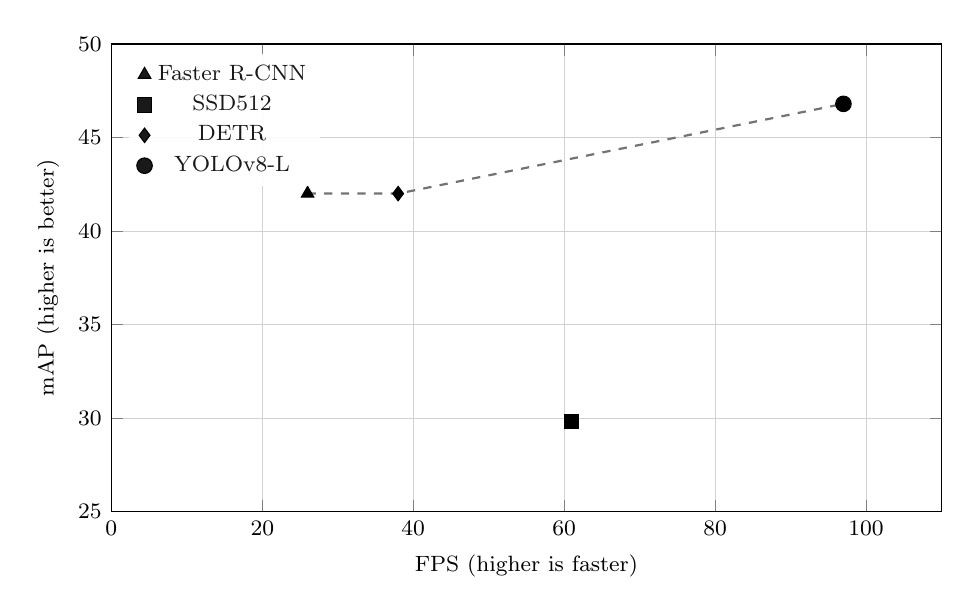
\begin{tikzpicture}
\begin{axis}[
    width=\columnwidth,
    height=0.62\columnwidth,
    grid=both,
    grid style={line width=.1pt, draw=gray!20},
    major grid style={line width=.2pt, draw=gray!35},
    xlabel={FPS (higher is faster)},
    ylabel={mAP (higher is better)},
    xmin=0, xmax=110,
    ymin=25, ymax=50,
    xtick={0,20,40,60,80,100},
    ytick={25,30,35,40,45,50},
    ticklabel style={font=\footnotesize},
    label style={font=\footnotesize},
    legend style={font=\footnotesize, at={(0.02,0.98)}, anchor=north west,
                  draw=none, fill=white, fill opacity=0.9},
]
% Points (FPS, mAP)
\addplot[only marks, mark=triangle*, mark size=2.6pt]
    coordinates {(26,42.0)};
\addlegendentry{Faster R-CNN}

\addplot[only marks, mark=square*, mark size=2.6pt]
    coordinates {(61,29.8)};
\addlegendentry{SSD512}

\addplot[only marks, mark=diamond*, mark size=2.6pt]
    coordinates {(38,42.0)};
\addlegendentry{DETR}

\addplot[only marks, mark=*, mark size=2.8pt]
    coordinates {(97,46.8)};
\addlegendentry{YOLOv8-L}

% A simple guide to the efficiency frontier (illustrative)
\addplot[thick, dashed, color=black!55]
    coordinates {(26,42.0) (38,42.0) (97,46.8)};
\end{axis}
\end{tikzpicture}
\caption{Illustrative accuracy--throughput map. The dashed line
is a visual guide to the current efficiency frontier for the
models in Table~\ref{tab:sota_compact}.}
\label{fig:pareto}
\end{figure}

The plotted grouping highlights the practical ceiling that has
driven detector evolution. Older efficient models tend to
cluster in the lower-right (fast but less accurate), while
high-precision multi-stage pipelines drift toward the upper-left
(accurate but slower). Recent optimized one-stage families,
typified by modern YOLO variants, attempt to move the frontier by
improving feature reuse, multi-scale learning, and training
stability without introducing heavy sequential stages. In this
sense, the Pareto view is not merely a visualization; it is a
design diagnostic: when a new method claims improvement, the
question is whether it moves the frontier outward or simply
shifts along it by trading speed for accuracy (or the reverse).

% ============================================================
% PAGE 9 — FUTURE DEVELOPMENTS AND EMERGING TRENDS
% Paste this BELOW Page 8 content and BEFORE \begin{thebibliography}
% ============================================================

\section{Future Developments and Emerging Trends}

Object detection has progressed from hand-crafted pipelines to
highly optimized deep models and, more recently, attention-based
set predictors. Yet the field remains in rapid motion, pushed
by deployment constraints (power, latency, privacy), new sensing
modalities (depth and multi-view), and expanding definitions of
``what counts as an object'' (open-vocabulary recognition). This
section highlights three directions that are likely to shape the
next generation of detectors.

\subsection{Edge AI and TinyML: Detection Under Tight Budgets}

A major practical frontier is shifting high-quality detection
from data centers to devices that operate under strict energy,
memory, and thermal limits: smartphones, wearable cameras,
drones, and IoT sensors. Running detection locally reduces
cloud dependency, improves privacy, and eliminates network
latency, but it introduces hard constraints that directly
challenge modern architectures: limited on-chip SRAM, slower
memory bandwidth, and reduced arithmetic throughput.

Progress here is increasingly driven by \textit{model
compression and co-design}. Common strategies include structured
pruning (removing channels or blocks rather than individual
weights), quantization-aware training for INT8/INT4 inference,
and knowledge distillation \cite{hinton2015distilling} to
transfer performance from a large teacher detector to a compact
student. In addition, hardware-aware neural architecture search
(NAS) \cite{wu2019fbnet} optimizes the network not for proxy
metrics such as FLOPs alone, but for measured latency on target
accelerators. The combined effect is a shift in evaluation
culture: detectors are increasingly judged by accuracy at a
given energy envelope or at a given on-device latency, not only
by mAP on a high-end GPU.

\subsection{3D Object Detection: From Boxes to Spatial Understanding}

Many safety-critical applications require not only 2D boxes but
3D spatial reasoning: the distance to a pedestrian, the yaw of a
vehicle, or the location of obstacles relative to a robot's
trajectory. 3D object detection expands the output space from
2D rectangles to 3D cuboids (position, size, and orientation),
often within a world coordinate frame. This introduces new
sources of complexity: depth ambiguity, calibration errors, and
occlusion across viewpoints.

LiDAR-camera fusion is a particularly active area because the
modalities are complementary. LiDAR provides accurate geometry
but sparse appearance cues; cameras provide dense semantics but
depth is implicit. Fusion architectures attempt to align these
signals either early (fusing features before heavy processing)
or late (combining modality-specific predictions). A prominent
trend is to use a \textit{Bird's-Eye View (BEV)} representation
as a unifying coordinate system, projecting multi-view camera
features and LiDAR points into a shared top-down plane before
detection \cite{liu2023bevfusion}. While BEV-based fusion can
improve robustness and planning relevance, it also highlights
engineering challenges: maintaining geometric consistency,
handling moving objects during sensor synchronization, and
ensuring stable performance under adverse weather or low-light
conditions.

\subsection{Self-Supervised and Open-Vocabulary Detection}

A second major trend is reducing the dependency on exhaustive
box-level annotations. Traditional detectors are trained on
fully labeled datasets where each object instance is boxed and
classified, which is expensive and difficult to scale across
domains. Self-supervised representation learning offers an
alternative: pretrain backbones on large unlabeled corpora and
fine-tune for detection with fewer labels. Methods such as
MoCo \cite{he2020momentum} and masked autoencoders (MAE)
\cite{he2022masked} have shown that strong visual features can
be learned without explicit category supervision, improving
sample efficiency and transfer to new domains.

In parallel, open-vocabulary detection aims to detect categories
that were not explicitly present during detector training by
connecting vision to language. Instead of fixing the label set
to the training taxonomy, the model conditions predictions on
text prompts or class names. Approaches such as GLIP
\cite{li2022glip} align region-level visual features with
language embeddings so that a detector can generalize to novel
object names at inference time. This reframes detection as a
\textit{grounding} problem: ``find regions that correspond to
this phrase.'' The technical challenge is to preserve the
localization quality and calibration of conventional detectors
while extending them to a dynamic, text-defined label space.
If successful, open-vocabulary detection could substantially
reduce the cost of deploying detectors in specialized settings
by replacing dataset re-labeling with prompt engineering and
targeted adaptation.

% ============================================================
% PAGE 10 — CONCLUSION AND REFERENCES
% Paste this BELOW Page 9 content.
% Then REPLACE your existing bibliography with the one below.
% If you use \balance, place it just before \begin{thebibliography}.
% ============================================================

\section{Conclusion}

This paper traced the evolution of object detection through the
lens of its defining constraint: the tension between
\textit{precision} and \textit{speed}. In the pre-deep-learning
era, detectors such as Viola--Jones, HOG+SVM pipelines, and
deformable part-based models achieved impressive results for
their time by pairing carefully engineered features with
computationally efficient search and scoring strategies. These
approaches proved that real-time detection was possible on
modest hardware, but their reliance on fixed descriptors
eventually imposed a representational ceiling as scenes grew
more diverse and benchmarks demanded robust generalization.

The deep learning shift replaced manual feature design with
learned representations. Two-stage detectors---R-CNN, Fast
R-CNN, and Faster R-CNN---pushed accuracy forward by separating
candidate generation from classification and box refinement,
and by progressively making the pipeline more shareable and
end-to-end trainable. In parallel, one-stage detectors
reframed detection as dense prediction, trading proposal stages
for single-pass throughput. The YOLO and SSD families made
real-time detection broadly practical, while innovations such
as Focal Loss (RetinaNet) addressed dense-classification
imbalances that previously limited one-stage mAP.

More recently, attention-based designs have expanded the
modeling toolkit. DETR demonstrated that detection can be cast
as direct set prediction with bipartite matching, removing the
need for anchors and NMS in principle. Hierarchical vision
transformers such as Swin brought improved computational
structure to attention, making transformer backbones more
compatible with multi-scale detection workloads.

A central takeaway is that the notion of a single ``best''
detector is no longer meaningful in isolation. The preferred
architecture depends on the deployment objective and
constraints: some settings demand maximum mAP and stable
localization under occlusion, while others prioritize FPS,
power, memory footprint, privacy, or on-device execution. Seen
this way, modern detector design is best understood as an
optimization problem over an application-specific point on the
speed--precision (and often energy) frontier. Progress occurs
when new ideas shift that frontier outward rather than merely
moving along it.

% ============================================================
% BALANCE COLUMNS ON LAST PAGE (optional but recommended)
% ============================================================
\balance

% ============================================================
% REFERENCES — comprehensive list for Pages 1–10
% ============================================================
\begin{thebibliography}{00}

\bibitem{viola2001rapid}
P.~Viola and M.~Jones, ``Rapid object detection using a boosted
cascade of simple features,'' in \textit{Proc. IEEE Conf. Comput.
Vis. Pattern Recognit. (CVPR)}, 2001, pp.~511--518.

\bibitem{viola2004robust}
P.~Viola and M.~Jones, ``Robust real-time face detection,''
\textit{Int. J. Comput. Vis.}, vol.~57, no.~2, pp.~137--154, 2004.

\bibitem{dalal2005histograms}
N.~Dalal and B.~Triggs, ``Histograms of oriented gradients for
human detection,'' in \textit{Proc. IEEE Conf. Comput. Vis. Pattern
Recognit. (CVPR)}, 2005, pp.~886--893.

\bibitem{felzenszwalb2010object}
P.~F. Felzenszwalb, R.~B. Girshick, D.~McAllester, and D.~Ramanan,
``Object detection with discriminatively trained part-based
models,'' \textit{IEEE Trans. Pattern Anal. Mach. Intell.},
vol.~32, no.~9, pp.~1627--1645, 2010.

\bibitem{krizhevsky2012imagenet}
A.~Krizhevsky, I.~Sutskever, and G.~E. Hinton,
``ImageNet classification with deep convolutional neural
networks,'' in \textit{Proc. NeurIPS}, 2012, pp.~1097--1105.

\bibitem{uijlings2013selective}
J.~R.~R. Uijlings, K.~E.~A. van~de~Sande, T.~Gevers, and
A.~W.~M. Smeulders, ``Selective search for object recognition,''
\textit{Int. J. Comput. Vis.}, vol.~104, no.~2, pp.~154--171, 2013.

\bibitem{girshick2014rich}
R.~Girshick, J.~Donahue, T.~Darrell, and J.~Malik,
``Rich feature hierarchies for accurate object detection and
semantic segmentation,'' in \textit{Proc. CVPR}, 2014,
pp.~580--587.

\bibitem{girshick2015fast}
R.~Girshick, ``Fast R-CNN,'' in \textit{Proc. ICCV}, 2015,
pp.~1440--1448.

\bibitem{ren2015faster}
S.~Ren, K.~He, R.~Girshick, and J.~Sun, ``Faster R-CNN:
Towards real-time object detection with region proposal
networks,'' in \textit{Proc. NeurIPS}, 2015, pp.~91--99.

\bibitem{redmon2016you}
J.~Redmon, S.~Divvala, R.~Girshick, and A.~Farhadi,
``You only look once: Unified, real-time object detection,''
in \textit{Proc. CVPR}, 2016, pp.~779--788.

\bibitem{liu2016ssd}
W.~Liu \textit{et al.}, ``SSD: Single shot multibox detector,''
in \textit{Proc. ECCV}, 2016, pp.~21--37.

\bibitem{redmon2017yolo9000}
J.~Redmon and A.~Farhadi, ``YOLO9000: Better, faster, stronger,''
in \textit{Proc. CVPR}, 2017, pp.~6517--6525.

\bibitem{lin2017feature}
T.~-Y. Lin, P.~Doll\'{a}r, R.~Girshick, K.~He,
B.~Hariharan, and S.~Belongie, ``Feature pyramid networks for
object detection,'' in \textit{Proc. CVPR}, 2017, pp.~2117--2125.

\bibitem{lin2017focal}
T.~-Y. Lin, P.~Goyal, R.~Girshick, K.~He, and
P.~Doll\'{a}r, ``Focal loss for dense object detection,''
in \textit{Proc. ICCV}, 2017, pp.~2980--2988.

\bibitem{redmon2018yolov3}
J.~Redmon and A.~Farhadi, ``YOLOv3: An incremental improvement,''
\textit{arXiv:1804.02767}, 2018.

\bibitem{bochkovskiy2020yolov4}
A.~Bochkovskiy, C.~-Y. Wang, and H.~-Y.~M. Liao,
``YOLOv4: Optimal speed and accuracy of object detection,''
\textit{arXiv:2004.10934}, 2020.

\bibitem{carion2020end}
N.~Carion \textit{et al.}, ``End-to-end object detection with
transformers,'' in \textit{Proc. ECCV}, 2020, pp.~213--229.

\bibitem{he2020momentum}
K.~He, H.~Fan, Y.~Wu, S.~Xie, and R.~Girshick,
``Momentum contrast for unsupervised visual representation
learning,'' in \textit{Proc. CVPR}, 2020, pp.~9729--9738.

\bibitem{wang2020cspnet}
C.~-Y. Wang \textit{et al.}, ``CSPNet: A new backbone that can
enhance learning capability of CNN,'' in \textit{Proc. CVPRW},
2020, pp.~390--391.

\bibitem{liu2021swin}
Z.~Liu \textit{et al.}, ``Swin Transformer: Hierarchical vision
transformer using shifted windows,'' in \textit{Proc. ICCV},
2021, pp.~10012--10022.

\bibitem{he2022masked}
K.~He \textit{et al.}, ``Masked autoencoders are scalable vision
learners,'' in \textit{Proc. CVPR}, 2022, pp.~16000--16009.

\bibitem{li2022glip}
L.~Li \textit{et al.}, ``Grounded language-image pre-training,''
in \textit{Proc. CVPR}, 2022, pp.~10965--10975.

\bibitem{wang2023yolov7}
C.~-Y. Wang, A.~Bochkovskiy, and H.~-Y.~M. Liao,
``YOLOv7: Trainable bag-of-freebies sets new state-of-the-art for
real-time object detectors,'' in \textit{Proc. CVPR}, 2023,
pp.~7464--7475.

\bibitem{liu2023bevfusion}
Z.~Liu \textit{et al.}, ``BEVFusion: Multi-task multi-sensor fusion
with unified bird's-eye view representation,'' in \textit{Proc. ICRA},
2023, pp.~2774--2781.

\bibitem{jocher2023yolov8}
G.~Jocher, A.~Chaurasia, and J.~Qiu, ``Ultralytics YOLOv8,'' 2023.
[Online]. Available: \url{https://github.com/ultralytics/ultralytics}

\bibitem{wu2019fbnet}
B.~Wu \textit{et al.}, ``FBNet: Hardware-aware efficient ConvNet
design via differentiable NAS,'' in \textit{Proc. CVPR}, 2019,
pp.~10734--10742.

\bibitem{hinton2015distilling}
G.~Hinton, O.~Vinyals, and J.~Dean, ``Distilling the knowledge in a
neural network,'' \textit{arXiv:1503.02531}, 2015.

\end{thebibliography}


\end{document}